\documentclass[a4paper, 12pt]{article}
\usepackage[left=2.5cm, right=2.5cm, top=3cm, bottom=3cm]{geometry}
\usepackage[spanish]{babel}
\usepackage{amsmath}
\usepackage{graphicx}
\usepackage{color}
\usepackage{xcolor}
\usepackage[utf8x]{inputenc}
\usepackage[T1]{fontenc}
\usepackage{listings}
\lstdefinelanguage{JavaScript}{
  keywords={break, case, catch, continue, debugger, default, delete, do, else, false, finally, for, function, if, in, instanceof, new, null, return, switch, this, throw, true, try, typeof, var, void, while, with},
  morecomment=[l]{//},
  morecomment=[s]{/*}{*/},
  morestring=[b]',
  morestring=[b]"
}
\usepackage{tikz}
\usetikzlibrary{shapes,arrows,positioning}
\usepackage{fancyhdr}
\usepackage{titlesec}
\usepackage{background}
\usepackage[hidelinks]{hyperref}
\usepackage{float}

\definecolor{colorgreen}{rgb}{0,0.6,0}
\definecolor{colorgray}{rgb}{0.5,0.5,0.5}
\definecolor{colorpurple}{rgb}{0.58,0,0.82}
\definecolor{colorback}{RGB}{255,255,204}
\definecolor{colorbackground}{RGB}{200,200,221}
\definecolor{bordercolor}{RGB}{0,0,128}

% Definiendo el estilo de las porciones de código
\lstset{
backgroundcolor=\color{colorbackground},
commentstyle=\color{colorgreen},
keywordstyle=\color{colorpurple},
numberstyle=\tiny\color{colorgray},
stringstyle=\color{colorgreen},
basicstyle=\ttfamily\footnotesize,
breakatwhitespace=false,
breaklines=true,
captionpos=b,
keepspaces=true,
numbers=left,
showspaces=false,
showstringspaces=false,
showtabs=false,
tabsize=2,
frame=single,
framesep=2pt,
rulecolor=\color{black},
framerule=1pt
}

% Configuración de encabezado y pie de página
\setlength{\headheight}{15.04742pt}
\addtolength{\topmargin}{-3.04742pt}
\pagestyle{fancy}
\fancyhf{}
\fancyhead[L]{\leftmark}
\fancyhead[R]{\thepage}
\fancyfoot[C]{\textit{Universidad de La Habana - Facultad de Matemática y Computación}}

% Configuración de títulos
\titleformat{\section}
  {\normalfont\Large\bfseries}{\thesection}{1em}{}
\titleformat{\subsection}
  {\normalfont\large\bfseries}{\thesubsection}{1em}{}

% Configuración de fondo de página
\backgroundsetup{
  scale=1,
  color=bordercolor,
  opacity=0.3,
  angle=0,
  position=current page.south,
  vshift=10cm,
  hshift=0cm,
  contents={%
    \begin{tikzpicture}[remember picture,overlay]
      \draw[bordercolor,ultra thick] (current page.south west) rectangle (current page.north east);
    \end{tikzpicture}
  }
}
%sl23

\begin{document}
\graphicspath{{./}}

\begin{titlepage}
    \centering
    \vspace*{2cm}
    {\huge\bfseries Informe\\[0.4cm]}
    {\LARGE HEX AI Player\\}
    \vspace*{2cm}
    
     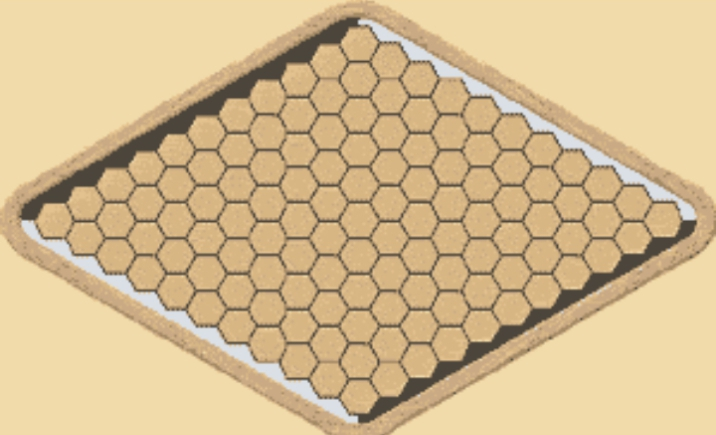
\includegraphics[width=0.5\textwidth, height=0.2\textheight]{Images/hextab.png}\\[0.5cm]
    {\Large \textbf{Richard Alejandro Matos Arderí}\\[0.5cm]}
    {\Large Grupo 311, Ciencia de la Computación\\[0.5cm]}
    {\Large Facultad de Matemática y Computación\\[0.5cm]}
    {\Large Universidad de La Habana\\[0.5cm]}
    \vfill
    
\includegraphics[width=0.2\textwidth, height=0.2\textheight]{Images/MATCOM.jpg}\\[0.5cm]
    {\Large 2025}
\end{titlepage}

\newpage
\tableofcontents
\newpage


\section{Implementación del Jugador Inteligente}

\subsection{Enfoque basado en Monte Carlo Tree Search}
Esta implementación de jugador inteligente para HEX utiliza una versión mejorada del algoritmo \textbf{Monte Carlo Tree Search (MCTS)}, siguiendo la estructura general del pseudocódigo presentado en el libro ``Inteligencia Artificial: Un enfoque moderno`` . El algoritmo se compone de cuatro fases principales:

\begin{enumerate}
	\item \textbf{Selección (SELECT)}: Recorre el árbol desde la raíz seleccionando nodos hijos según el criterio UCB1 hasta llegar a un nodo hoja.
	\item \textbf{Expansión (EXPAND)}: Crea uno o más nodos hijos a partir del nodo hoja si el juego no ha terminado.
	\item \textbf{Simulación (SIMULATE)}: Juega una partida aleatoria o semi-aleatoria desde el nuevo nodo hasta alcanzar un estado terminal.
	\item \textbf{Retropropagación (BACK-PROPAGATE)}: Actualiza las estadísticas de victorias y visitas en todos los nodos del camino recorrido.
\end{enumerate}

\begin{figure}[h]
	\centering
	\begin{verbatim}
		function MONTE-CARLO-TREE-SEARCH(state) returns an action
		tree ← NODE(state)
		while IS-TIME-REMAINING() do
			leaf ← SELECT(tree)
			child ← EXPAND(leaf)
			result ← SIMULATE(child)
			BACK-PROPAGATE(result, child)
		return the move in ACTIONS(state) whose node has highest number of playouts
	\end{verbatim}
	\caption{Pseudocódigo de MCTS adaptado de ``Inteligencia Artificial: Un enfoque moderno``}
	\label{fig:mcts-pseudo}
\end{figure}


\newpage

\section{Mejoras Implementadas}
La implementación extiende el MCTS básico con varias mejoras clave:

\subsection{Selección Heurística de Movimientos}
En la fase de expansión, en lugar de seleccionar movimientos puramente al azar, es utilizada una función heurística combinada que evalúa:

\begin{itemize}
	\item Distancia del camino más corto a la victoria (Dijkstra)
	\item Patrones estratégicos (puentes)
	\item Control del centro del tablero
	\item Conectividad de grupos
	\item Movilidad potencial
	\item Proximidad a bordes estratégicos
\end{itemize}

\begin{lstlisting}[language=Python,caption=Función de expansión heurística]
	def select_heuristic_move(self) -> tuple:
		moves = self.untried_moves
		move_scores = [(self._heuristic_score(move), move) for move in moves]
		move_scores.sort(reverse=True, key=lambda x: x[0])
		return move_scores[0][1]
\end{lstlisting}

\subsection{Simulación Informada}
La fase de simulación utiliza políticas heurísticas en lugar de movimientos aleatorios, lo que produce estimaciones de valor más precisas:

\begin{lstlisting}[language=Python,caption=Simulación basada en heurísticas]
	def _simulate(self, node: EnhancedMCTSNode) -> float:
	temp_board = node.board.clone()
	current_player = node.player_id
	steps = 0
	max_steps = temp_board.size * 2
	
	while steps < max_steps:
		if temp_board.check_connection(current_player):
			return 1.0 if current_player == self.player_id else 0.0
		moves = temp_board.get_possible_moves()
		move_scores = [(node._heuristic_score(move), move) for move in moves]
		best_move = max(move_scores, key=lambda x: x[0])[1]
		temp_board.place_piece(*best_move, current_player)
		current_player = 3 - current_player
		steps += 1
	return 0.5
\end{lstlisting}

\subsection{Estructura de Datos}
El árbol MCTS se implementa mediante la clase \texttt{EnhancedMCTSNode}, que almacena:

\begin{itemize}
	\item Estado del tablero (clonable)
	\item Movimiento que llevó a este nodo
	\item Estadísticas de visitas y victorias
	\item Hijos expandidos
	\item Movimientos no probados
	\item ID del jugador actual
\end{itemize}

\begin{lstlisting}[language=Python,caption=Estructura del nodo MCTS]
	class EnhancedMCTSNode:
		def __init__(self, board: HexBoard, parent=None, move=None, player_id: int = 1):
			self.board = board.clone()
			self.parent = parent
			self.move = move
			self.children: List[EnhancedMCTSNode] = []
			self.wins = 0
			self.visits = 0
			self.untried_moves = board.get_possible_moves()
			self.player_id = player_id
\end{lstlisting}

\subsection{Control de Tiempo}
El algoritmo ejecuta iteraciones MCTS dentro del límite de tiempo asignado (por defecto 9 segundos), reservando 0.1 segundos para la selección final del mejor movimiento:

\begin{lstlisting}[language=Python,caption=Bucle principal de búsqueda]
	while time.time() - start_time < self.time_limit - 0.1:
		node = self._select(root)
		if not node.is_terminal():
			node = node.expand()
		result = self._simulate(node)
		self._backpropagate(node, result)
		iterations += 1
\end{lstlisting}


\end{document}












































